\chapter{Fundamentação Teórica}

Neste capítulo, são descritos e detalhados os conceitos fundamentais e as ferramentas utilizadas durante a execução deste estudo. Inicialmente, procurou-se uma compreensão mais profunda das definições de acessibilidade, acessibilidade digital e acessibilidade universal, conceitos essenciais para a compreensão do escopo deste trabalho.

Em seguida, se realiza uma discussão acerca das vantagens advindas da incorporação da acessibilidade digital no processo de desenvolvimento de aplicações destinadas a dispositivos móveis.

Destaca-se a relevância deste aspecto e o impacto positivo que pode exercer sobre a experiência do usuário final. Visando também trazer uma compreensão das definições e impactos legais que a acessibilidade digital tem para os desenvolvedores, são discutidas as principais legislações vigentes no Brasil voltadas a defesa das PCD. 

Adicionalmente serão tratados quais as principais deficiências motoras, auditivas e visuais que afetam a população mundial, qual o impacto dela na vida dos portadores e quais os benefícios e relação da acessibilidade digital com a sua inclusão na sociedade.

Posteriormente, são apresentadas as tecnologias que se fizeram necessárias para a condução do desenvolvimento deste projeto. Nesta parte, dá-se ênfase à importância dos testes automatizados, procedimento que se revela fundamental para garantir a qualidade e efetividade das implementações realizadas.

Além disso, são discutidas as tecnologias específicas empregadas na elaboração de uma extensão para o Flutter que permita a análise estática de regras de acessibilidade em aplicações móveis desenvolvidas com este framework.

\section{Acessibilidade}

Conforme dados do Censo 2010 (IBGE, 2010), aproximadamente 46 milhões de brasileiros declararam ter algum grau de dificuldade em pelo menos uma das seguintes habilidades: enxergar, ouvir, caminhar ou subir degraus. Dessas, a habilidade de enxergar e ouvir são primordiais para a inclusão digital dos usuários. Portanto, se faz necessária a compreensão do conceito de acessibilidade, sua importância no mundo digital, o que pode ser implementado para melhorá-la e as respectivas questões legislativas aplicadas no Brasil.

\subsection{Definição de Acessibilidade}

A acessibilidade é um princípio fundamental que visa garantir a todos os indivíduos, independentemente de suas limitações físicas, sensoriais, intelectuais ou psicossociais, a capacidade de acessar e utilizar adequadamente um produto, serviço ou ambiente. Neste estudo, o foco se volta à acessibilidade no âmbito digital, especialmente em relação aos dispositivos móveis.

Entretanto, é necessário que compreender que a acessibilidade é para todos, e que atos ou soluções simples, tem um grande impacto na qualidade de vida das pessoas. Assim como define Kalbag (2017) “acessibilidade no mundo físico, é o nível em que um ambiente é utilizável pelo maior número de pessoas possíveis”.

Sendo assim, é simples compreender a importância e benefícios da acessibilidade no mundo físico. Kalbag (2017) traz um excelente exemplo de uma mudança de acessibilidade que estamos tendo em nosso mundo e acabamos por nem perceber o seu real impacto. Conforme na figura 2, é possível visualizar que maçanetas pivotantes podem ser abertas facilmente com um movimento vertical para baixo, mesmo que tenham algum grau de deficiência motora, pois podem utilizar seu corpo ou outros objetos como apoio para realizarem a abertura da porta. A princípio, esse exemplo parece não ter muita conexão com o mundo digital, porém podemos utilizá-lo como uma base para refletir a forma que construímos nossa interface, onde adicionamos complicações visando a estética, ou então apenas por decisão de produto, mas que podem ter um impacto negativo na usabilidade de PCD.

\begin{figure}[!h]
	\centering
	\caption{"Maçanetas pivotantes (à esquerda) só requerem um leve empurrão por cima. Maçanetas esféricas (à direita) necessitam de um movimento de torção com firmeza.”}
	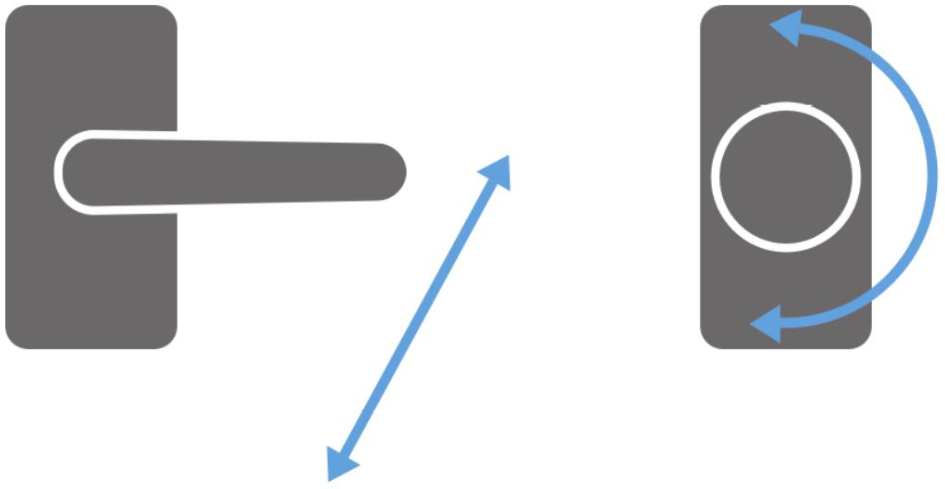
\includegraphics[width=256pt]{Assets/Macanetas pivotantes.png}
	\fonte{KALBAG. P. 11. (2017)}
\end{figure}

\subsection{Acessibilidade Universal}

\subsection{Acessibilidade Digital}

\subsection{Legislação Brasileira}

A Lei Brasileira de Inclusão (LBI), também conhecida como Estatuto da Pessoa com Deficiência (Lei Nº 13.146, de 6 de Julho de 2015), é um marco legal que busca assegurar e promover, em condições de igualdade, o exercício dos direitos e das liberdades fundamentais por pessoa com deficiência, visando à sua inclusão social e cidadania.

A LBI aborda várias áreas importantes para a inclusão, incluindo a acessibilidade, que tem implicações diretas para a concepção e desenvolvimento de dispositivos móveis. Ela define acessibilidade como sendo a possibilidade e condição de alcance para utilização, com segurança e autonomia, de espaços, mobiliários, equipamentos urbanos, edificações, transportes, informação e comunicação, inclusive seus sistemas e tecnologias, bem como de outros serviços e instalações abertos ao público, de uso público ou privados de uso coletivo, tanto na zona urbana como na rural, por pessoa com deficiência ou com mobilidade reduzida.

Nesse contexto, a LBI define no Art. 3º inciso um que Acessibilidade é a “possibilidade e condição de alcance para utilização, com segurança e autonomia, de espaços, mobiliários, equipamentos urbanos, edificações, transportes, informação e comunicação, inclusive seus sistemas e tecnologias, bem como de outros serviços e instalações abertos ao público, de uso público ou privados de uso coletivo, tanto na zona urbana como na rural, por pessoa com deficiência ou com mobilidade reduzida”. (BRASIL, 2015).

Adicionalmente, ela também define o que são tecnologias assistiva sou ajuda técnica no inciso três do Artigo 3 como sendo a “equipamentos, dispositivos, recursos, metodologias, estratégias, práticas e serviços que objetivem promover a funcionalidade, relacionada à atividade e à participação da pessoa com deficiência ou com mobilidade reduzida, visando à sua autonomia, independência, qualidade de vida e inclusão social” (BRASIL, 2015).

O Capítulo II da LBI descreve quais os direitos de pessoas com deficiência. E no contexto das aplicações móveis temos no Art. 9º que a “disponibilização de recursos, tanto humanos quanto tecnológicos, que garantam atendimento em igualdade de condições com as demais pessoas.” (BRASIL, 2015). Dessa forma é claro a necessidade de adequar as aplicações móveis para que não haja penalidades conforme descrito no Artigo 88 da LDI aos desenvolvedores no tangente a criação de barreiras para pessoas com deficiência.

Além da LBI, o Brasil conta com outras legislações voltadas à inclusão digital e à garantia dos direitos das pessoas com deficiência. Dentre elas, destacam-se o Decreto Nº 5.296 de 2 de dezembro de 2004, que regulamenta as Leis nº 10.048 e 10.098 e estabelece normas e critérios para a promoção de acessibilidade das pessoas com deficiência, e a Lei Nº 12.965, de 23 de abril de 2014, mais conhecida como Marco Civil da Internet, que estabelece princípios, garantias, direitos e deveres para o uso da Internet no Brasil.

\section{Pessoa com Deficiência}

\subsection{Deficiências motoras}

\subsection{Deficiências visuais}

\subsection{Deficiências auditivas}

\section{Flutter}

Flutter é uma estrutura de desenvolvimento de aplicativo que usa a linguagem de programação Dart. Ela permite a criação de interfaces de usuário altamente personalizáveis e expressivas com um bom desempenho. Ao contrário de outras estruturas de desenvolvimento móvel, como o React Native, Flutter não usa pontes de JavaScript, mas compila o código diretamente no código nativo do sistema operacional, o que melhora o desempenho (Google, 2023).

Sendo assim, segundo a mantenedora o Flutter oferece melhor desempenho, capacidade de “Hot Reload” permitindo que os desenvolvedores experimentem e construam interfaces mais rapidamente, Personalização através de um rico conjunto de “Widgets” --- os “blocos de construção” do Flutter --- seguindo inicialmente diretrizes do Material Design para Android e Cupertino para iOS mas sem bloquear modificações do desenvolvedor e também, permite o desenvolvimento de aplicativos para diferentes plataformas partindo de uma única fonte de código.

\section{Análise Estática de Código}

Ademais, o Flutter oferece uma série de recursos que ajudam os desenvolvedores a criar aplicativos acessíveis. Ela suporta APIs de acessibilidade para Android e iOS, incluindo a API TalkBack para Android e a API VoiceOver para iOS. Além disso, o Flutter tem suporte para ampliação de tela, fontes maiores, contraste de cores suficiente e navegação por teclado (Flutter, 2023). Entretanto ainda necessitam que o desenvolvedor utilize das ferramentas providas para criar aplicações realmente acessíveis.

\subsection{Acessibilidade}

\subsection{iOS e Android}

\section{Análise Estática de Código}
